\newpage
\section{Application Layer}
\subsection{Overview of application layer}
Builds distributed ``network services'' (DNS, Web) on transport services

\begin{figure}[!htb]
    \centering
    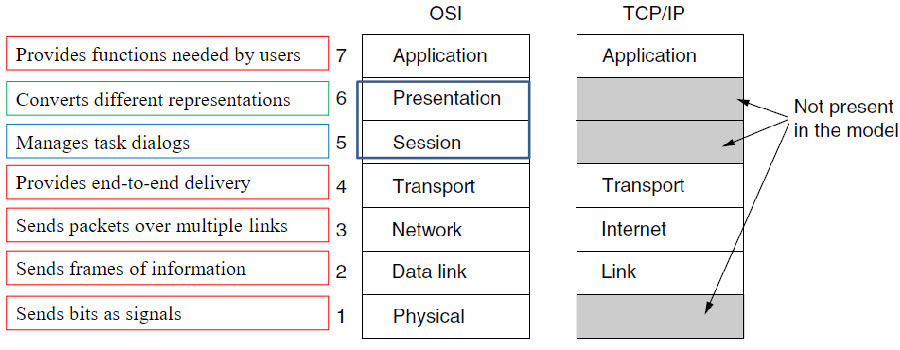
\includegraphics[width=0.42\textwidth]{pic/CN7/Presentation Layers}
    \caption{Presentation Layers}
\end{figure}

\subsubsection{Applications and Application Level Protocols}
The three concepts:
\begin{itemize}
    \item Service model
    \item Protocol
    \item Interface
\end{itemize}

Network application contains Client site, Server site, Application level protocol

\subsubsection{Parameters}
\begin{itemize}
    \item Data Loss
    \item Bandwidth
    \item Timing
\end{itemize}

\subsection{Important application layer protocols}

\subsubsection{DNS (Domain Name System)}
decouple machines names from machine addresses. 

The essence of DNS is the invention of a hierarchical, domain-based naming scheme and a distributed database system for implementing converting the machine names to network addresses. an application program calls a library procedure called the resolver. 

The query and response messages are sent as UDP packets. (现在不一定了, 不过书上是这样写的, 考试要这样答)

Why Not Centric:
\begin{itemize}
    \item Single point of failure
    \item Traffic volume
    \item Distant name server means slow response
    \item Scalability
\end{itemize}

\begin{figure}[!htb]
    \centering
    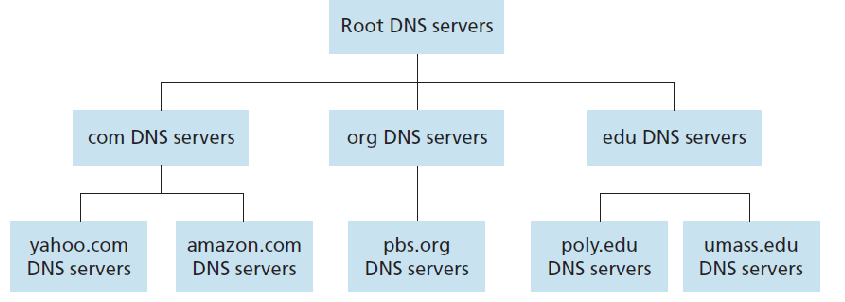
\includegraphics[width=0.42\textwidth]{pic/CN7/Portion of the hierarchy of DNS servers}
    \caption{Portion of the hierarchy of DNS servers}
\end{figure}


\paragraph{Root Nameservers}Root (dot) is served by 13 server names
\begin{itemize}
    \item a.root-servers.net to m.root-servers.net
    \item Each ``server'' is actually a cluster of replicated servers, for both security and reliability purposes
\end{itemize}

\begin{figure}[!htb]
    \centering
    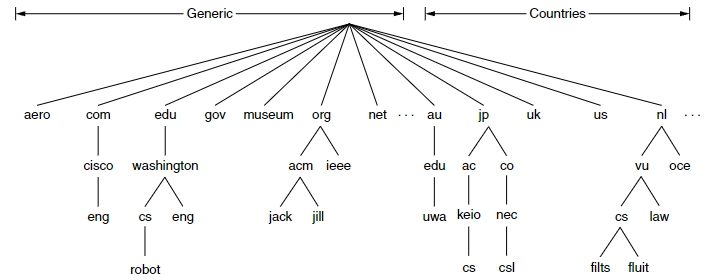
\includegraphics[width=0.42\textwidth]{pic/CN7/A portion of the Internet domain name space.}
    \caption{A portion of the Internet domain name space.}
\end{figure}

TLDs (Top-Level Domains) Run by ICANN. 

\paragraph{DNS Zones}Each zone has one or more nameservers to contact for
information about it.

\paragraph{Domain Resource Records}The primary function of DNS is to map domain names onto resource records.

A resource record is a five-tuple. The format is as follows:
\begin{itemize}
    \item Domain name: This field is thus the primary search key used to satisfy queries
    \item Time to live: how stable the record is. 
    \item Class: For Internet information, it is always IN
    \item Type
    \begin{figure}[!htb]
        \centering
        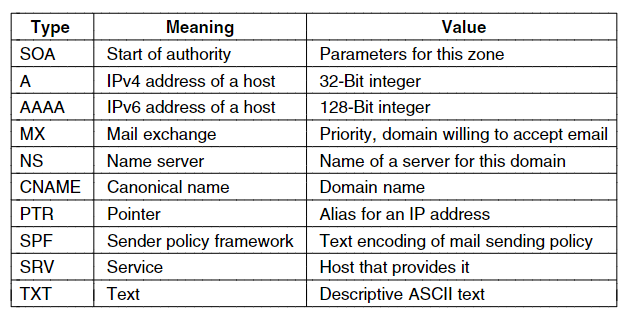
\includegraphics[width=0.42\textwidth]{pic/CN7/The principal DNS resource record types.}
        \caption{The principal DNS resource record types.}
    \end{figure}
    \begin{itemize}\scriptsize
        \item An SOA record provides the name of the primary source of information about the name server's zone.
        \item A: 32-bit IPv4 address
        \item AAAA: 128-bit IPv6 address
        \item MX: it specifies the name of the host prepared to accept email for the specific domain
        \item NS: a name server
        \item CNAME: ppt 参考文献 [7]
        \item PTR: allow lookups of the IP address and return the name of the corresponding machine. -- reverse lookups
        \item SRV: a newer type of record that allows a host to be identified for a given service in a domain. 
        \item SPF: This helps receiving machines check that mail is valid.
        \item TXT: 
    \end{itemize}
    \item Value
\end{itemize}

\paragraph{DNS Resolution}DNS protocol lets a host resolve any host name (domain) to IP address. 

\begin{figure}[!htb]
    \centering
    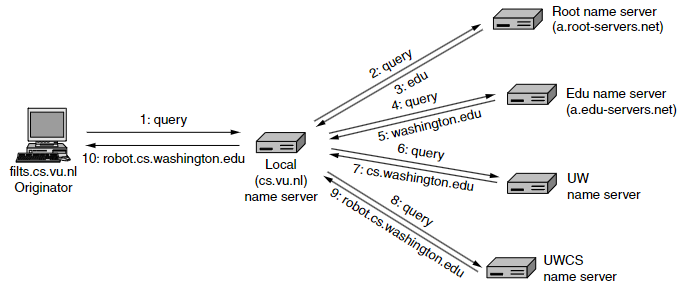
\includegraphics[width=0.42\textwidth]{pic/CN7/Example of a resolver looking up a remote name in 10 steps.}
    \caption{Example of a resolver looking up a remote name in 10 steps.}
\end{figure}

\paragraph{Iterative vs. Recursive Queries}\quad
\begin{itemize}\small
    \item Recursive query: Nameserver completes resolution and returns the final answer (客户端 -- 本地 DNS 服务器)
    \item Iterative query: Nameserver returns the answer or who to contact next for the answer (本地 DNS 服务器 -- 外网)
\end{itemize}

\paragraph{DNS Caching vs. Freshness}Information is cached between 5 minutes and 72 hours

\paragraph{Local Nameservers}Local nameservers typically run by IT

\paragraph{Name Servers}There are 13 root DNS servers. Most of the root servers are
present in multiple geographical locations and reached using
anycast routing, in which a packet is delivered to the nearest
instance of a destination address.

\paragraph{DNS Protocol}Query and response messages are Built on UDP messages, port 53. Service reliability via replicas. Security is a major issue. 

\paragraph{Security of DNS}\quad
Initially, the transaction ID was only 16 bits. This design choice left DNS vulnerable to a variety attacks including ``cache poisoning attack''. (伪造 DNS)

\begin{figure}[!htb]
    \centering
    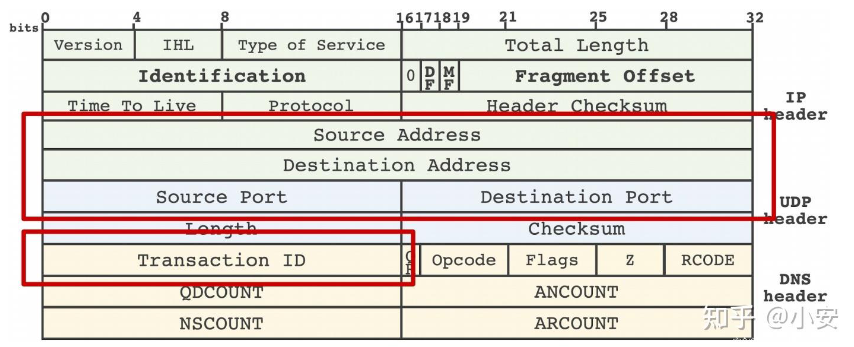
\includegraphics[width=0.42\textwidth]{pic/CN7/DNS Header}
    \caption{DNS Header}
\end{figure}

\begin{itemize}
    \item Oblivious DNS
    \item DNSsec
\end{itemize}

\subsubsection{FTP(File Transfer)}
FTP: to transfer files to and from a remote host. 

Steps:
\begin{enumerate}
    \item The user first provides the hostname of the remote host, causing
    the FTP client process in the local host to establish a TCP
    connection with the FTP server process in the remote host.
    \item The user then provides the user identification and password,
    which are sent over the TCP connection as part of FTP commands.
    \item Once the server has authorized the user, the user copies one or
    more files stored in the local file system into the remote file system
    (or vice versa).
\end{enumerate}

FTP uses two parallel TCP connections to transfer a file, a
control connection and a data connection.

\subsubsection{Email(Electronic Mail)}
Email is an asynchronous communication medium

Three major components:
\begin{enumerate}
    \item User agents
    \item Message transfer agents (mail servers)
    \item Simple mail transfer protocol: SMTP
\end{enumerate}

\begin{figure}[!htb]
    \centering
    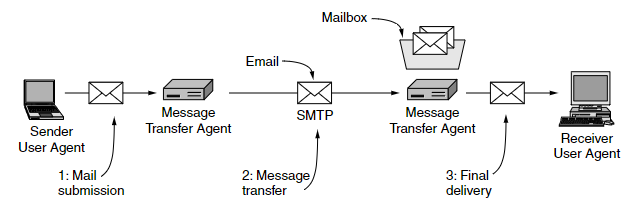
\includegraphics[width=0.42\textwidth]{pic/CN7/Architecture of the email system.}
    \caption{Architecture of the email system.}
\end{figure}

\paragraph{SMTP} is the principal application layer protocol for Internet electronic mail

\paragraph{MIME}The Multimedia Internet Mail Extension

\paragraph{Mail Access Protocols}SMTP has been designed for pushing email form one host to another. obtaining the messages is a pull operation,
whereas SMTP is a push protocol

Final Delivery:
\begin{itemize}
    \item POP
    \item IMAP
    \item HTTP
\end{itemize}

\subsubsection{HTTP(The HyperText Transfer Protocol)}
The HTTP, the Web's application-layer protocol, is at the heart of the
Web.

HTTP is a simple request-response protocol that normally runs over
TCP. HTTP has nothing to do with how a Web page is interpreted by a client.


Web page as a set of related Web resources  The content from these different servers is integrated for display by the browser.

HTTP is a request/response protocol for fetching Web resources

\paragraph{Fetching a Web page with HTTP}\quad
the Client Side

Steps:
\begin{enumerate}
    \item Resolve the server to IP address (DNS)
    \item Set up TCP connection to the server
    \item Send HTTP request for the page
    \item (Await HTTP response for the page)
    \item Execute / fetch embedded resources /render (不只是展示网页中内容,可能还要运行程序等。)
    \item Clean up an idle TCP connections
\end{enumerate}

The Server Side

Steps:
\begin{enumerate}
    \item Accept a TCP connection from a client (a browser).
    \item Get the path to the page, which is the name of the file requested.
    \item Get the file (from disk).
    \item Send the contents of the file to the client.
    \item Release the TCP connection.
\end{enumerate}

\paragraph{Cookies}It remembers stateful information for the stateless HTTP protocol

A cookie may contain up to five fields:
\begin{enumerate}
    \item The Domain tells where the cookie came from
    \item The Path is a path in the server’s directory structure that identifies
    which parts of the server’s file tree may use the cookie.
    \item The Content field is where the cookie’s content is stored.
    \item The Expires field specifies when the cookie expires
    \item The Secure field can be sent to indicate that the browser may only
    return the cookie to a server using a secure transport. This feature
    is used for e-commerce.
\end{enumerate}

%TODO ?-112

\paragraph{HTTP Message Format}\quad %TODO 113

Request

Request Headers

Example

Response

Example

\paragraph{html}需要记 html 一些语法. %TODO 148

css


\paragraph{Dynamic Web Pages}也会考